\chapter{Introduction} \label{chap:intro}

\lipsum[1-1]
Example cite \cite{lee2020vector}.

\section{Motivation}


\begin{figure}
  \centering
  \begin{subfigure}[b]{0.40\linewidth}
    \centering
    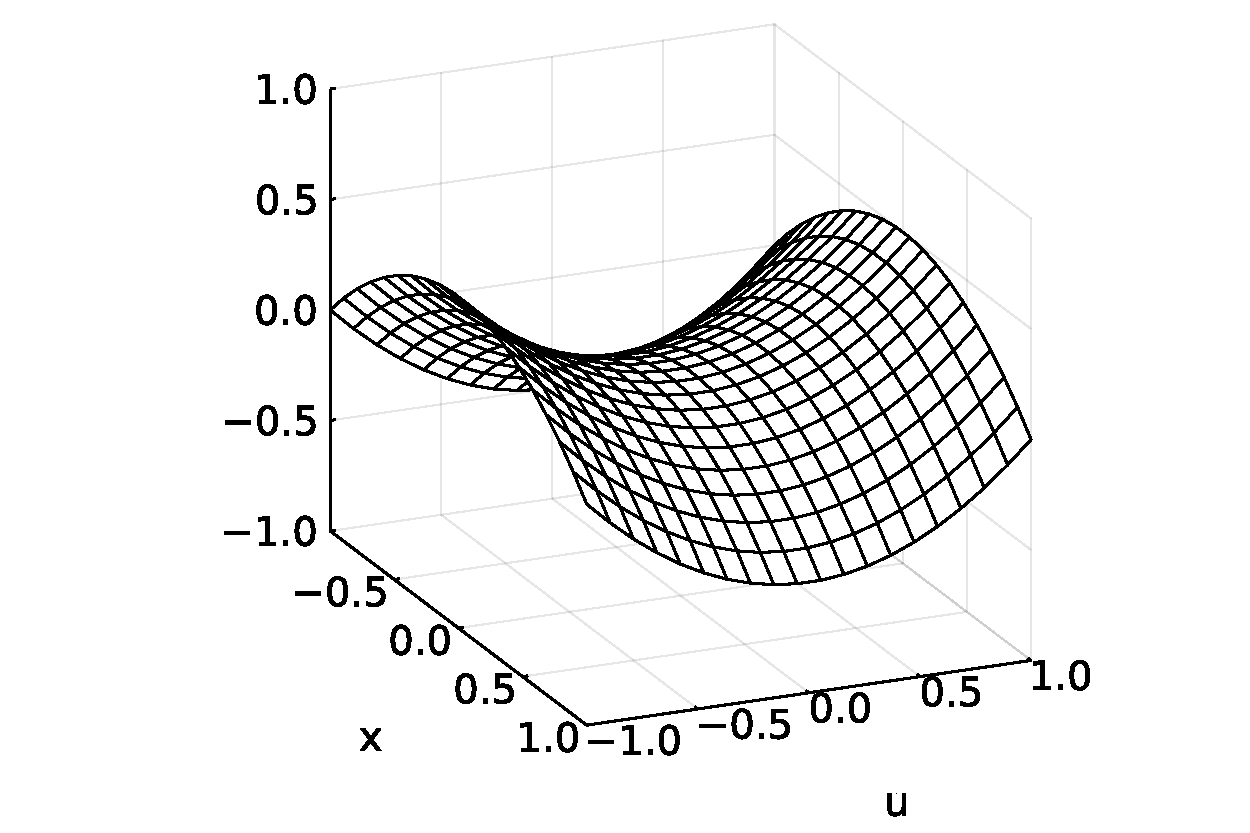
\includegraphics[width=1.0\linewidth]{./figures/first.pdf}
    \caption{First}
  \end{subfigure}
  \begin{subfigure}[b]{0.40\linewidth}
    \centering
    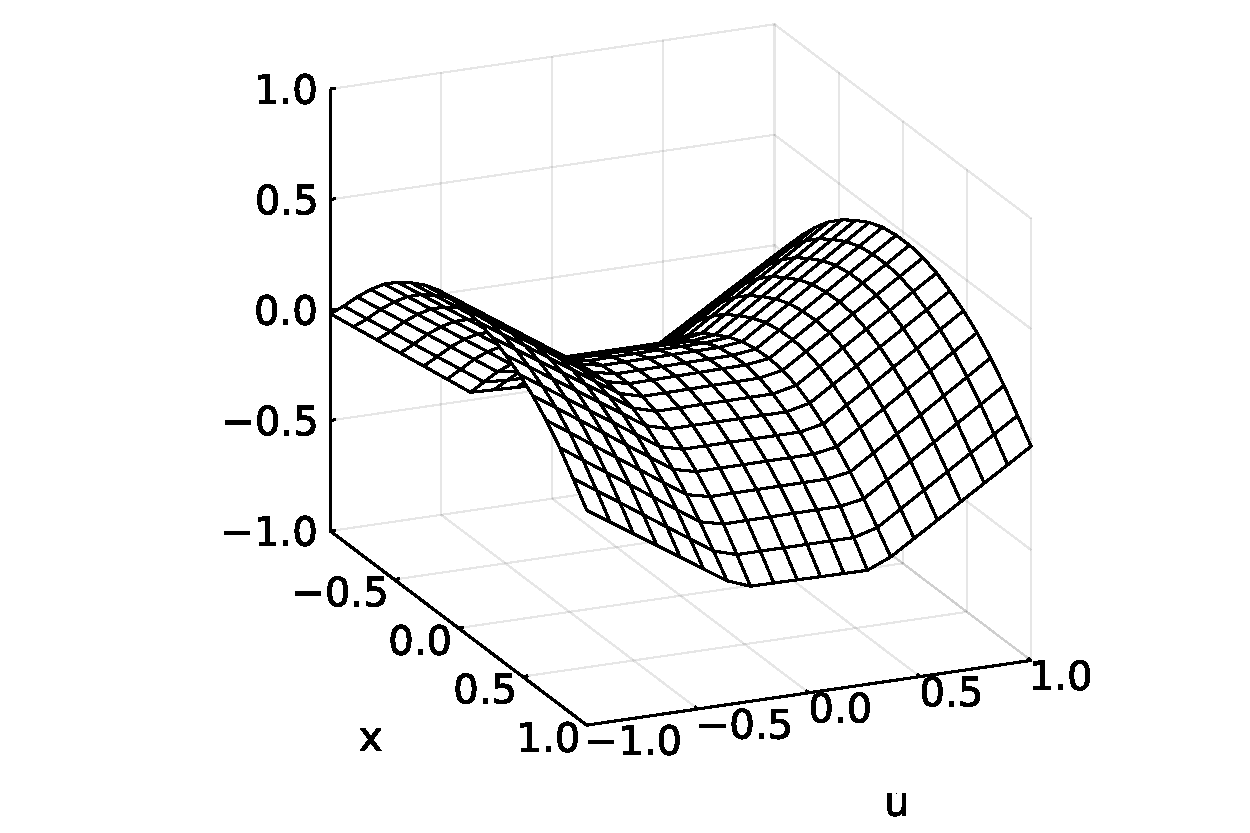
\includegraphics[width=1.0\linewidth]{./figures/second.pdf}
    \caption{Second}
  \end{subfigure}

  \caption{Subfigure example~\cite{kimParameterizedConvexUniversal2022}}
  \label{fig:subfigure_example}
\end{figure}

\lipsum[2-5]
